%=======================================================
%	PACKAGES AND THEMES
%=======================================================
\documentclass[8pt]{beamer}
\mode<presentation> {
\usepackage{etex}
\usetheme{Boadilla}
\definecolor{navyblue}{rgb}{0.0, 0.0, 0.5}
\definecolor{dkgreen}{rgb}{0,0.6,0}
\definecolor{gray}{RGB}{64, 64, 64}
\definecolor{mauve}{rgb}{0.58,0,0.82}
\usecolortheme[named = navyblue]{structure}
\setbeamercolor{normal text}{fg = gray}
\setbeamercolor{frametitle}{fg = white, bg = navyblue}
\setbeamerfont{framesubtitle}{size = \normalsize}
\setbeamerfont{caption}{size=\footnotesize}
\setbeamercolor{page number in head/foot}{fg = gray}
\setbeamertemplate{footline}%[frame number]
}


\usepackage{graphicx} % Allows including images
\usepackage{booktabs} % Allows the use of \toprule, \midrule and \bottomrule in tables
\usepackage{multicol}
\usepackage[export]{adjustbox}
\usepackage{colortbl}
\usepackage{graphicx} 

\usepackage{tikz}
\usepackage{fancybox}
\usepackage[absolute, overlay]{textpos}
\usepackage{multirow}
\usepackage{siunitx}
\usepackage{tcolorbox}


\usepackage{tikz}
\usepackage{calc}
\newlength{\outerradius}
\newlength{\innerradius}
\setlength{\outerradius}{0.50cm}
\setlength{\innerradius}{0.35cm}

%Damit wir Quellcode nutzen können.
\usepackage{listings}
\lstset{numbers=left,
	numberstyle=\tiny,
	numbersep=5pt,
	breaklines=true,
	showstringspaces=false,
	frame=l ,
	xleftmargin=15pt,
	xrightmargin=15pt,
	basicstyle=\ttfamily\scriptsize,
	stepnumber=1,
	keywordstyle=\color{blue},          % keyword style
  	commentstyle=\color{dkgreen},       % comment style
  	stringstyle=\color{mauve}         % string literal style
}
%Sprache Festelegen
\lstset{language=R}


%=======================================================
%	TITLE PAGE
%=======================================================

\title{\textbf{Innovation Networks}}

\author{Dr Daniele Rotolo}

\institute
{
SPRU (Science Policy Research Unit) \\
Business School\\
University of Sussex \\

\medskip

\medskip

\medskip

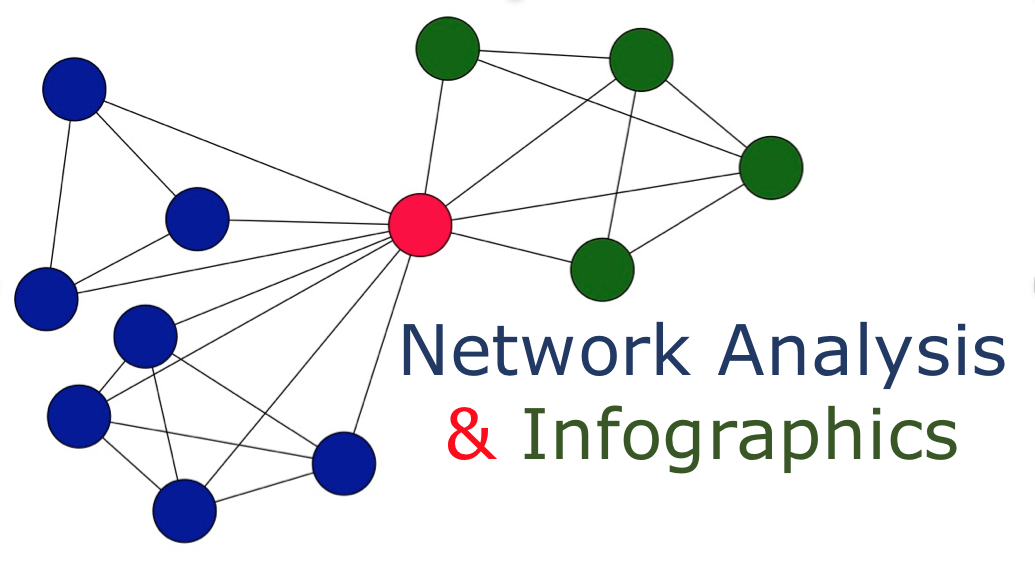
\includegraphics[width=2.5cm]{../_shared_pics/logo}

\medskip

\textit{{\color{dkgreen}{Week 9}}}\\
}


\date{} % Date, can be changed to a custom date

\begin{document}

\begin{frame}
\titlepage % Print the title page as the first slide

\begin{textblock*}{10pt}(0pt, 0.9\textheight)

\includegraphics[width=4cm]{../_shared_pics/SPRU.png}
\end{textblock*}

\end{frame}


%=======================================================
%	Learning outcomes
%=======================================================

\begin{frame}
\frametitle{Learning Outcomes}

\centering
\footnotesize
\begin{tabular}{lp{5.5cm}l}
\toprule
\multicolumn{2}{l}{\textbf{Learning outcome}} & \textbf{Assessment mode}\\
\hline
\\
1 & 
Explain the concept of network and list the main network indicators & 
ESS\\
\\
\rowcolor{green!20}2 & 
Describe and apply the major techniques for the collection of network data and their statistical analysis & 
ESS, GPN + GWS\\
\\
\rowcolor{green!20}3 & 
Identify the main characteristics of networks by means of network measures  & 
ESS, GPN + GWS\\
\\
4 &
Employ network analysis techniques to produce network data-based infographics & 
GPN + GWS\\
\\
\bottomrule
\multicolumn{3}{l}{Note: ESS: Essay; GPN: Group Presentation; GWS: Group Written Submission}\\
\end{tabular}

\end{frame}

%------------------------------------------------






%=======================================================
%	Intro slides
%=======================================================
\section*{Overview}
%------------------------------------------------

\begin{frame}
\frametitle{\insertsection}
\tableofcontents[hideallsubsections]
\end{frame}

%------------------------------------------------







%=======================================================	
% Bibliometrics/scientometrics
%=======================================================
\section{Bibliometrics/scientometrics}

%------------------------------------------------

\bgroup
\setbeamercolor{background canvas}{bg = navyblue}
\begin{frame}[plain]{}
\begin{center}
\color{white}{\Huge\insertsection}
\end{center}
\end{frame}
\egroup

%------------------------------------------------

\begin{frame}
\frametitle{\insertsection}
\framesubtitle{Definition}

\begin{columns}[c]

\column{.45\textwidth}
\begin{itemize}
\item {\color{blue}{Scientometrics}} is ``the quantitative study of science, communication in science, and science policy'' \cite{Hess1997}

\item {\color{blue}{Bibliometrics}} is ``the measurement of patterns in written communication'' \cite{Broadus1987}

\item \textit{Bibliometrics in not restricted to scientific communication, while scientometrics is not restricted to bibliometric measures}

\item {\color{blue}{Related sub-disciplines}}: informetrics, technometrics, research evaluation, altmetrics

\end{itemize}   

\column{.45\textwidth}
\centering
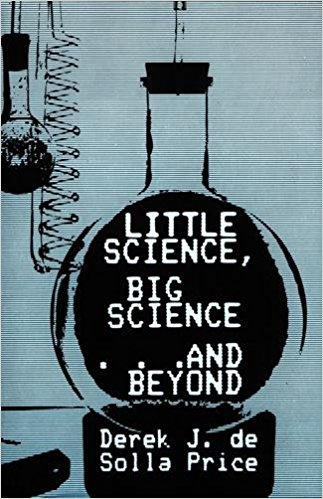
\includegraphics[height=0.7\textheight]{price}\\    
\tiny{\cite{DeSollaPrice1963}}
 
\end{columns}

\end{frame}

%------------------------------------------------

\begin{frame}
\frametitle{\insertsection}
\framesubtitle{Unit of analysis}

\begin{columns}[c]

\column{.50\textwidth}
{\color{blue}{Documents}} are the main source of data
\begin{itemize}
\item publications
\item patents
\item news articles
\item ...
\end{itemize}

\column{.45\textwidth}
\end{columns}

\begin{textblock*}{8cm}(7cm, 1.5cm)
\colorbox{white}{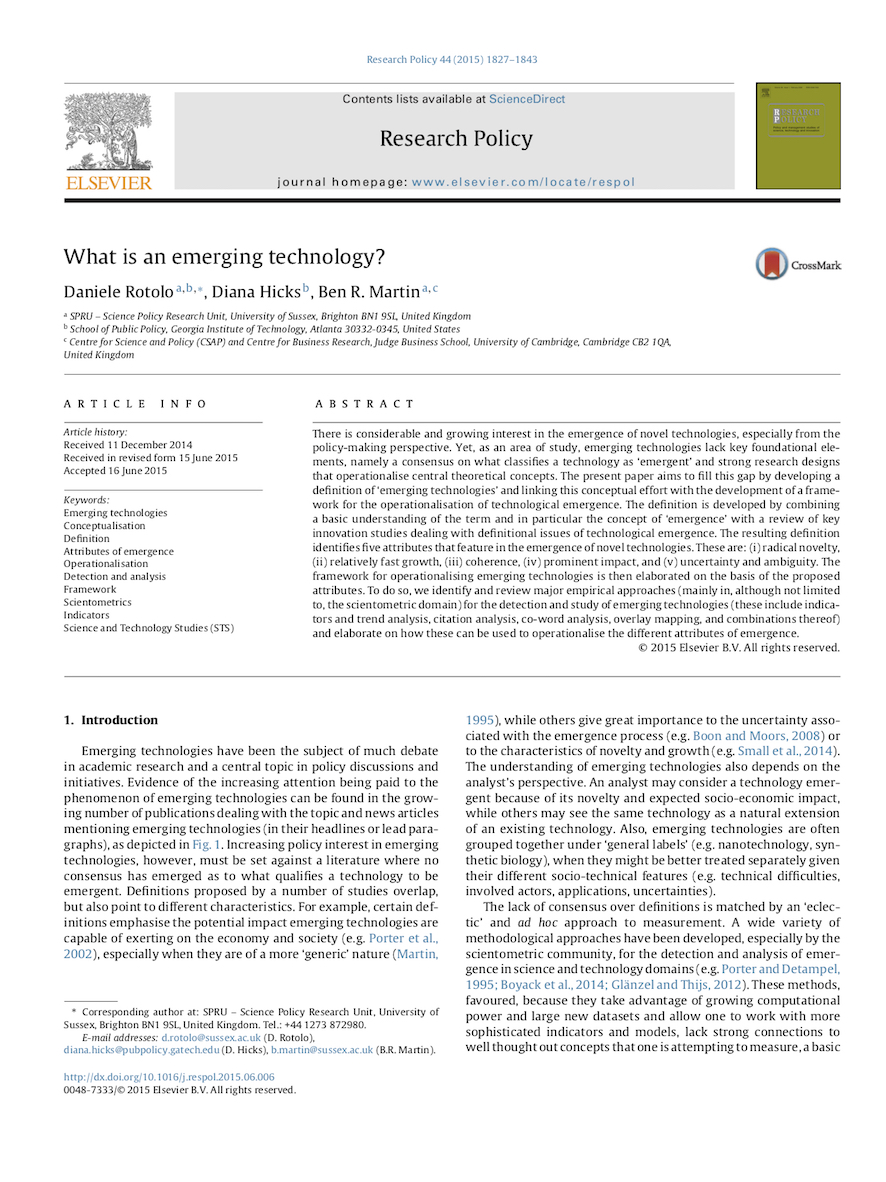
\includegraphics[width=4cm, frame]{paper}}
\end{textblock*}

\begin{textblock*}{8cm}(8cm, 3.5cm)
\colorbox{white}{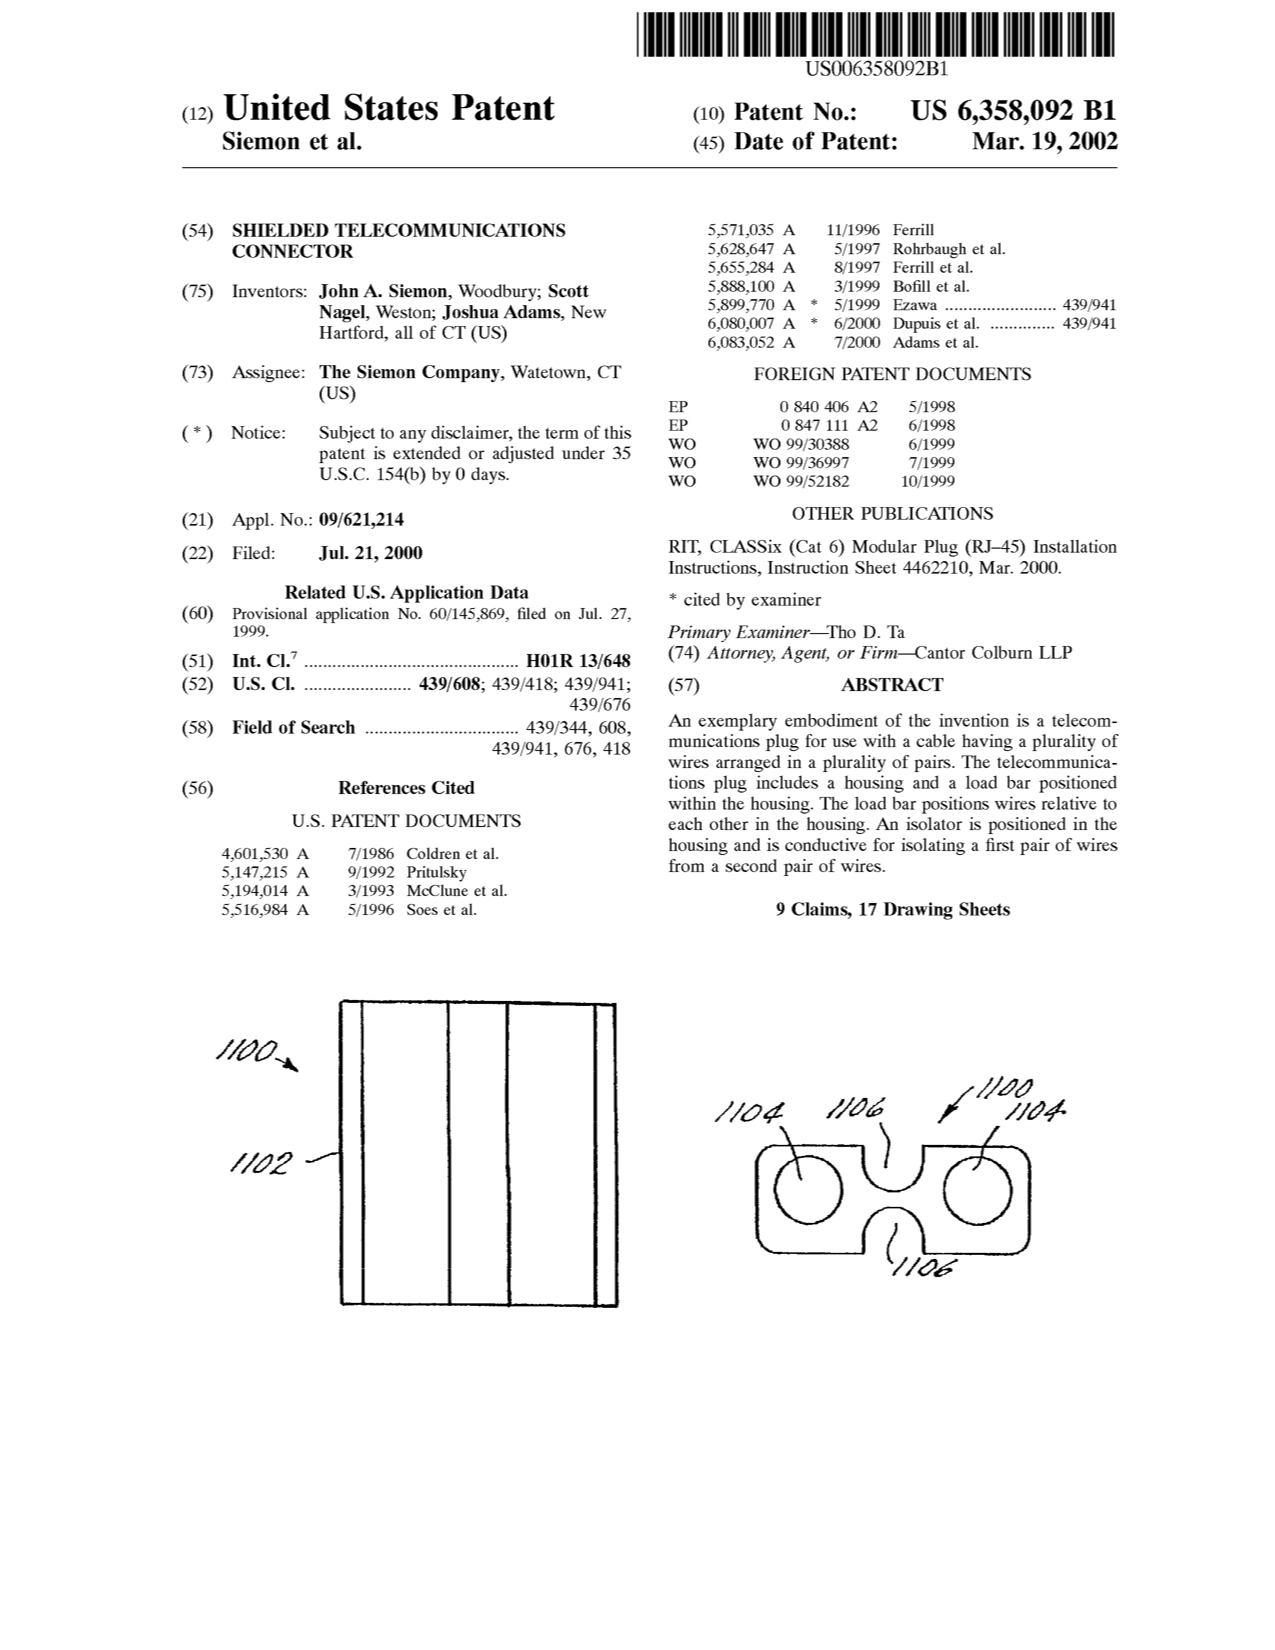
\includegraphics[width=4cm, frame]{patent}}
\end{textblock*}

\end{frame}

%------------------------------------------------

\begin{frame}
\frametitle{\insertsection}
\framesubtitle{Focus}

\begin{itemize}
\item Measurement of {\color{blue}{impact}} (e.g.\ citation count, h-index, impact factor)
\item Understanding of {\color{blue}{citation behavior}} (e.g.\ norms)
\item {\color{blue}{Normalisation}} (e.g.\ comparison across research areas)
\item Development of {\color{blue}{indicators}} to support decision making (e.g.\ funding)
\item {\color{blue}{Mapping}} of science and technology
\end{itemize}

\end{frame}

%------------------------------------------------

\begin{frame}
\frametitle{\insertsection}
\framesubtitle{Mapping}


Network analysis has been extensively used in {\color{blue}{bibliometrics/scientometrics}} to map science and technology \cite{Rotolo2015b}

\begin{itemize}
\item Mapping of collaboration
\item Mapping of cognitive connections
\end{itemize}

\end{frame}

%------------------------------------------------




%=======================================================	
% Mapping of collaboration
%=======================================================
\section{Mapping of collaboration}
%------------------------------------------------

\bgroup
\setbeamercolor{background canvas}{bg = navyblue}
\begin{frame}[plain]{}
\begin{center}
\color{white}{\Huge\insertsection}
\end{center}
\end{frame}
\egroup

%------------------------------------------------

\begin{frame}
\frametitle{\insertsection}
\framesubtitle{Publication data and co-authorship}

\begin{columns}[c]

\column{.3\textwidth}

\onslide<2>{
\begin{itemize}
\item Authors
\item Organisations
\item Cities
\item Countries
\end{itemize}
}

\column{.7\textwidth}
\centering
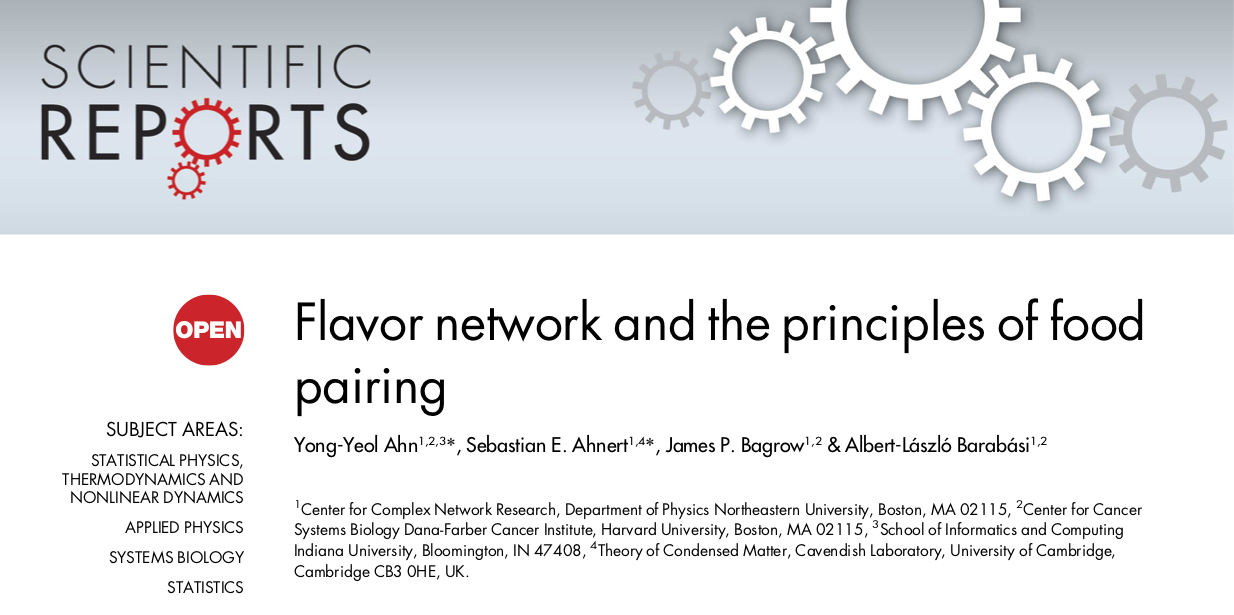
\includegraphics[width=8cm, frame]{paper_collaboration}\\     
\tiny{Source: \cite{Ahn2011}}

\end{columns}

\end{frame}

%------------------------------------------------

\begin{frame}
\frametitle{\insertsection}
\framesubtitle{Publication data and co-authorship}

\begin{columns}[c]

\column{.45\textwidth}
\centering
\textit{Wide format}

\begin{table}
\begin{tabular}{|l|l|}
\hline
Publication  & Authors \\
\hline
PUB1       & AU1, AU2\\
PUB2       & AU1, AU3 \\
PUB3       & AU3, AU4, AU5\\
...          & ...\\
\hline
\end{tabular}
\end{table}

\column{.45\textwidth}

\onslide<2>{
\centering
\textit{Long format}

\begin{table}
\begin{tabular}{|l|l|}
\hline
Publication  & Author \\
\hline
PUB1       & AU1\\
PUB1       & AU2\\
PUB2       & AU1\\
PUB2       & AU3\\
PUB3       & AU3\\
PUB3       & AU4\\
PUB3       & AU5\\
...          & ...\\
\hline
\end{tabular}
\end{table}
}

\end{columns}



\end{frame}

%------------------------------------------------

\begin{frame}
\frametitle{\insertsection}
\framesubtitle{Publication data and co-authorship}

\centering
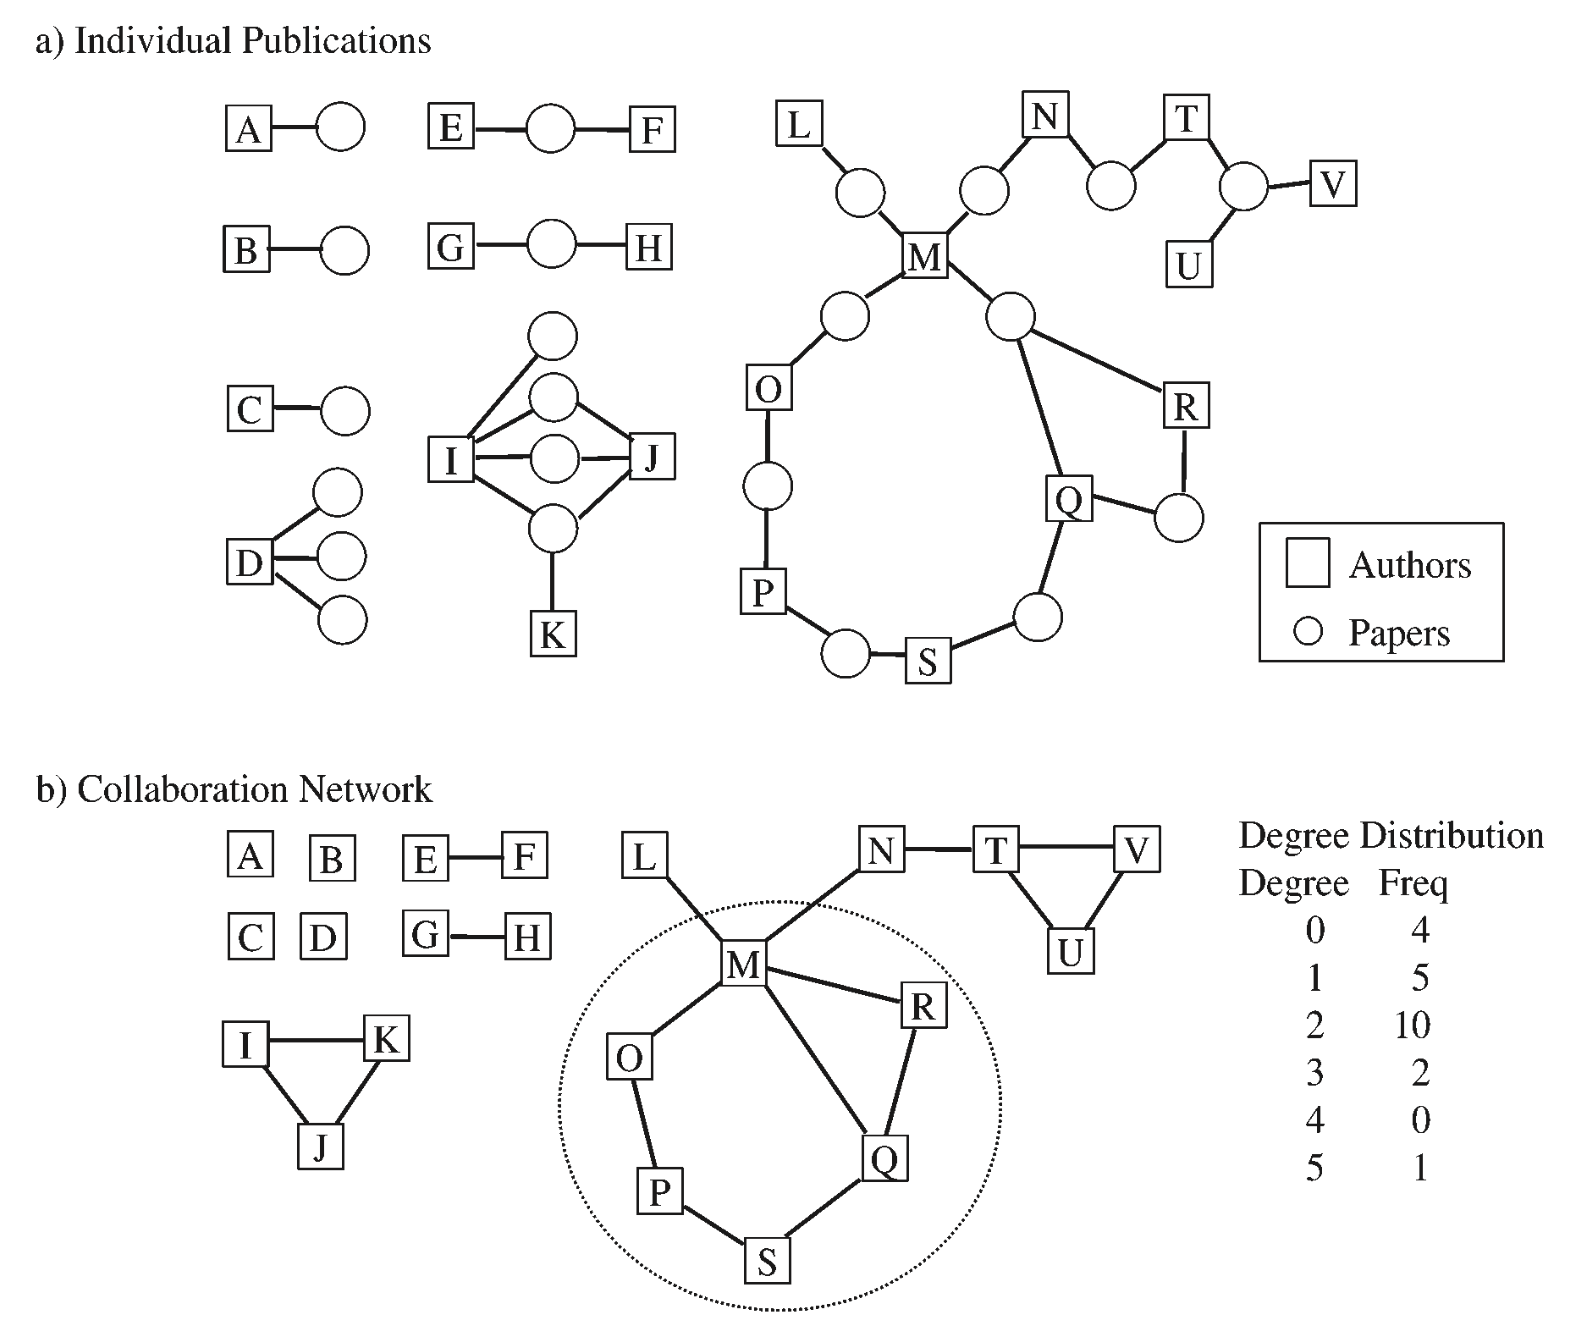
\includegraphics[height=0.75\textheight]{construction}\\     
\tiny{Source: Construction of the co-authorship network \cite{Moody2004}}


\end{frame}

%------------------------------------------------

\begin{frame}
\frametitle{\insertsection}
\framesubtitle{Publication data and co-authorship}

\begin{columns}[c]

\column{.45\textwidth}
{\color{blue}{Pioneering studies}} on co-authorship
\begin{itemize}
\item Increasing collaboration \cite{DeSollaPrice1963}
\item Structure and change of collaborative networks \cite{Melin1996}
\item Giant component, strength of collaboration, small-world \cite{Newman2001a}
\item Preferential attachment \cite{Albert2002}
\item ...
\end{itemize}

\column{.45\textwidth}
\centering
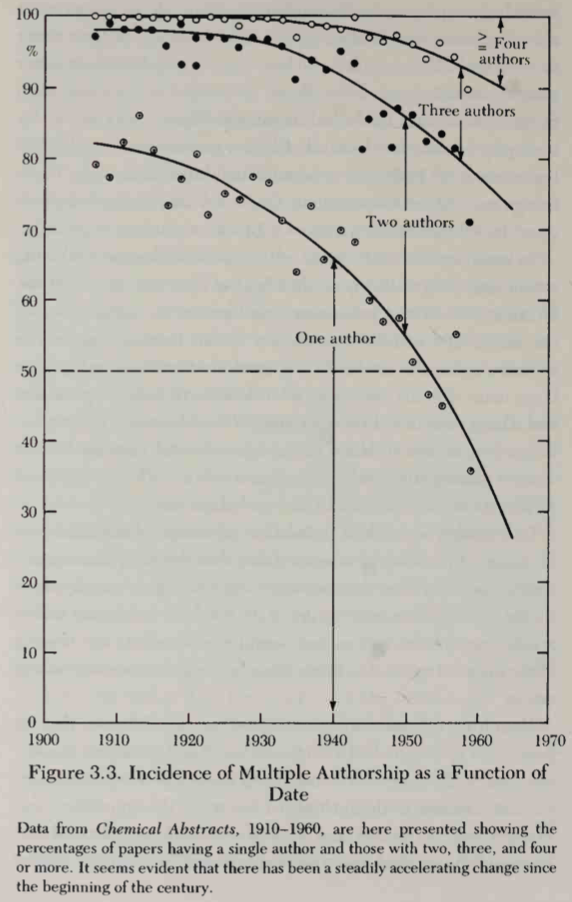
\includegraphics[height=0.8\textheight]{invisible_college}\\     
\tiny{Source: Invisible colleges \cite{DeSollaPrice1963}}

\end{columns}


\end{frame}

%------------------------------------------------

\begin{frame}
\frametitle{\insertsection}
\framesubtitle{Publication data and co-authorship (example)}

\textbf{Microneedles}: needles the size of which is on the \textit{micrometer} length scale. Expected impact on vaccines, drug delivery, and reduction of biohazard waste
   
\begin{columns}

\column{.45\textwidth}
\begin{minipage}[c][.6\textheight][c]{\linewidth}
\centering
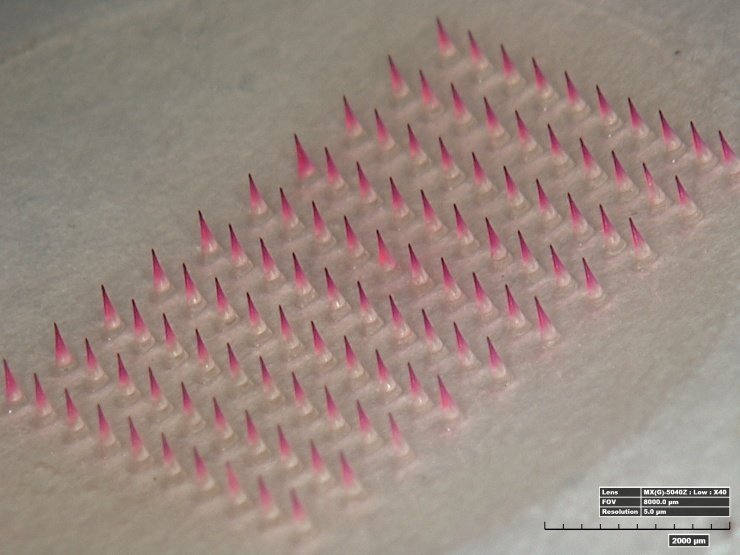
\includegraphics[width=0.8\textwidth,keepaspectratio]{micro1}\\
\tiny{Source: \url{www.news.gatech.edu}}	 	
\end{minipage}
        
\column{.45\textwidth}
\begin{minipage}[c][.6\textheight][c]{\linewidth}
\centering
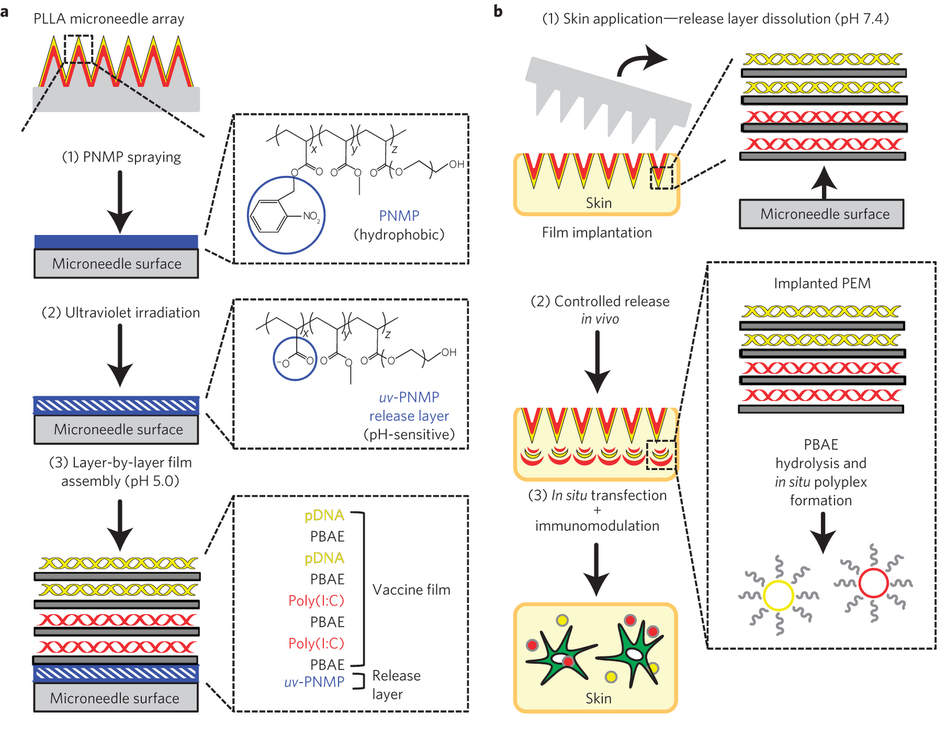
\includegraphics[width=0.8\textwidth,keepaspectratio]{micro2}\\
\tiny{Source: \cite{DeMuth2013}}	
\end{minipage}

\end{columns}

\end{frame}

%------------------------------------------------

\bgroup
\setbeamercolor{background canvas}{bg=black}
\begin{frame}[plain]{}
\centering{
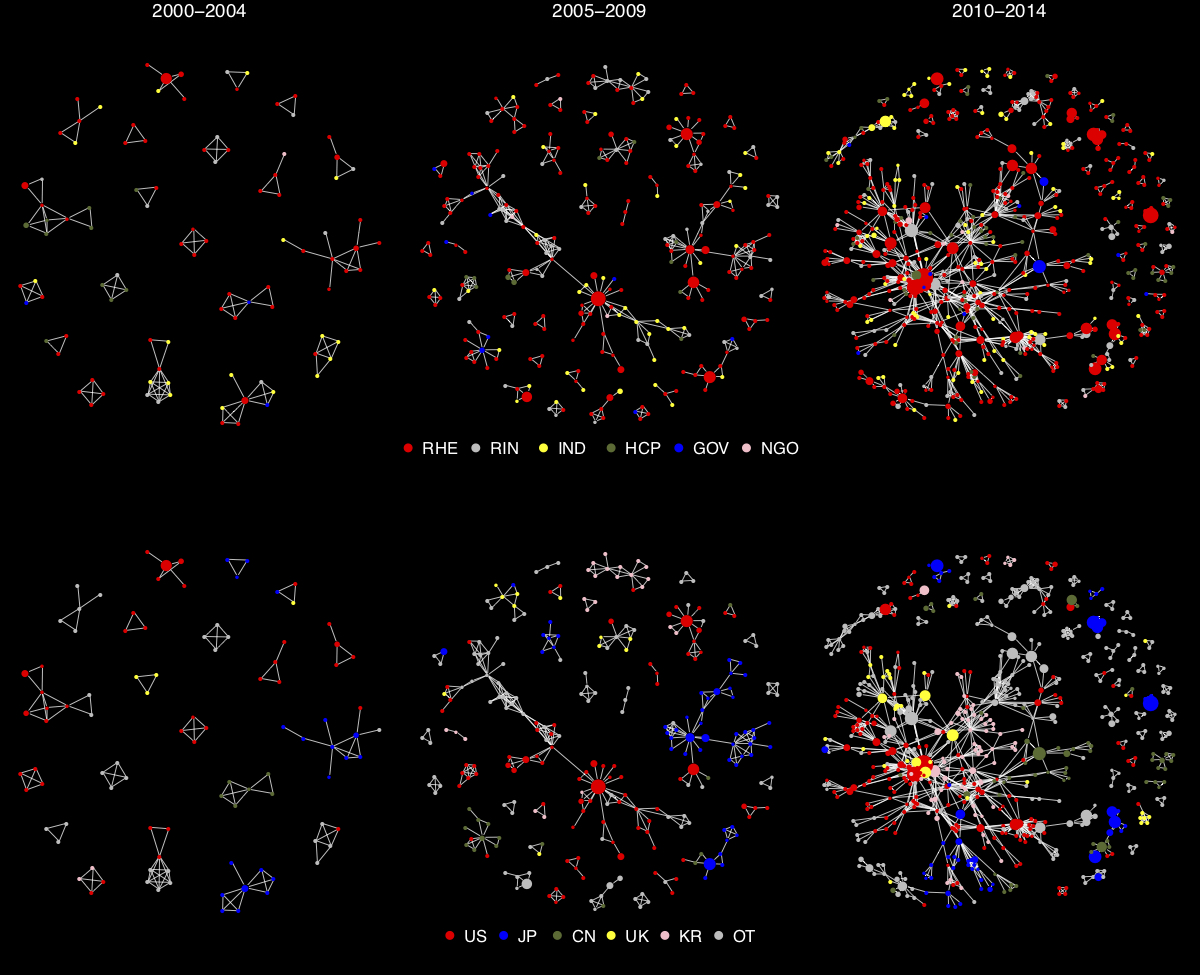
\includegraphics[width=0.85\paperwidth]{network_dynamics}}\\
\tiny{{\color{white}{Source: Co-authorship data in microneedles research (2000-2014)}}}
\end{frame}
\egroup

%------------------------------------------------


\begin{frame}
\frametitle{\insertsection}
\framesubtitle{Publication data and co-authorship}


\begin{columns}[c]

\column{.45\textwidth}
\centering

\begin{table}
\begin{tabular}{|l|l|}
\hline
Publication  & Authors \\
\hline
PUB1       & AU1, AU2\\
PUB2       & AU1, AU3 \\
PUB3       & AU3, AU4, AU5\\
...        & ...\\
\hline
\end{tabular}
\end{table}

\column{.45\textwidth}
\centering
When using co-authorship data to map collaboration networks, \\
do we make any {\color{red}{assumption}}?

\end{columns}

\end{frame}

%------------------------------------------------
\begin{frame}
\frametitle{\insertsection}
\framesubtitle{Publication data and co-authorship}

\centering
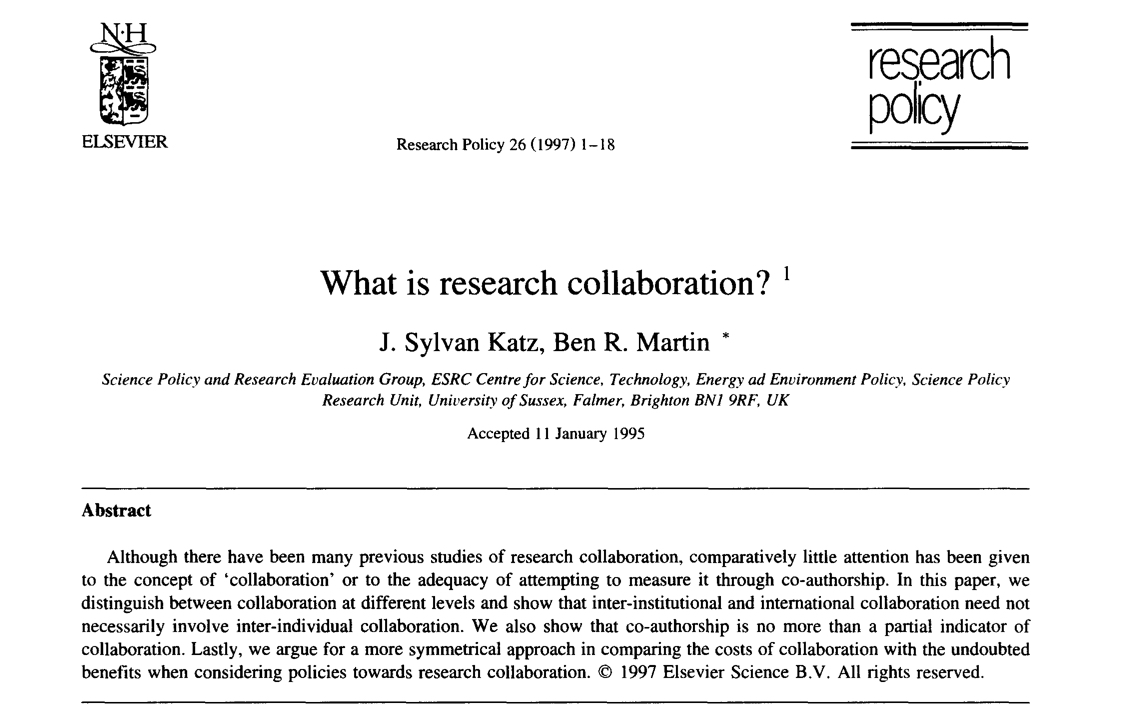
\includegraphics[height=0.6\textheight, frame]{katz}\\
\tiny{Source: \cite{Katz1997}}  
   
\end{frame}

%------------------------------------------------

\begin{frame}
\frametitle{\insertsection}
\framesubtitle{Patent data and co-authorship}

\begin{columns}[c]

\column{.3\textwidth}
\onslide<2>{\begin{itemize}
\item Inventors
\item Organisations
\item Cities
\item Countries
\item {\color{red}{Assumptions}}}
\end{itemize}

\column{.7\textwidth}
\centering
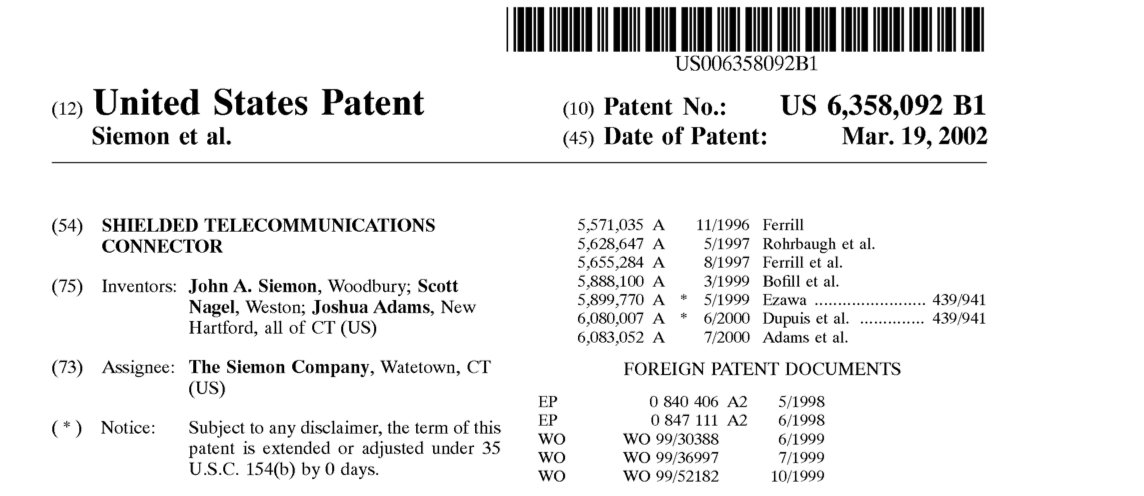
\includegraphics[width=8cm,, frame]{patent_collaboration}\\     
\tiny{Source: Patent US 6,358,092}

\end{columns}

\end{frame}

%------------------------------------------------

\begin{frame}
\frametitle{\insertsection}
\framesubtitle{Patent data and co-authorship (example)}

\begin{columns}[c]

\column{.45\textwidth}
\centering
Tesla\\
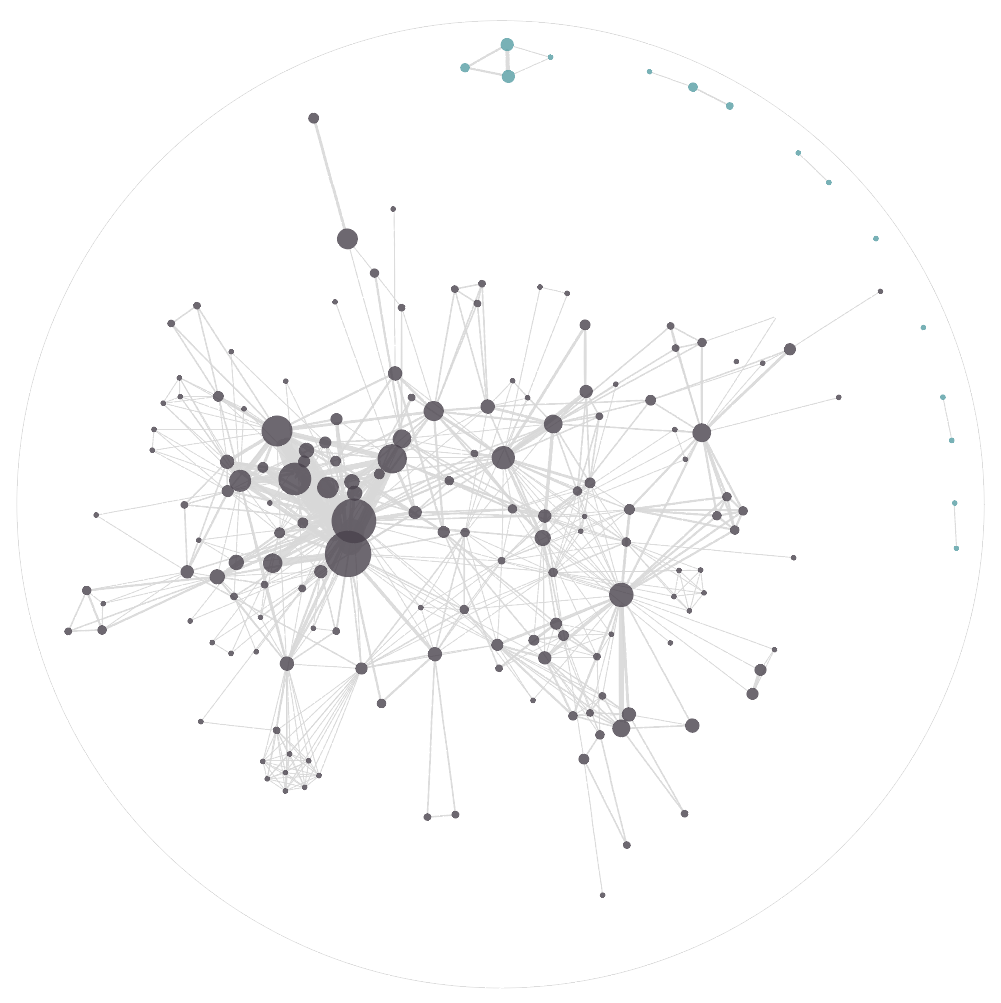
\includegraphics[width=6cm]{tesla_patents}

\column{.45\textwidth}
\centering
Facebook\\
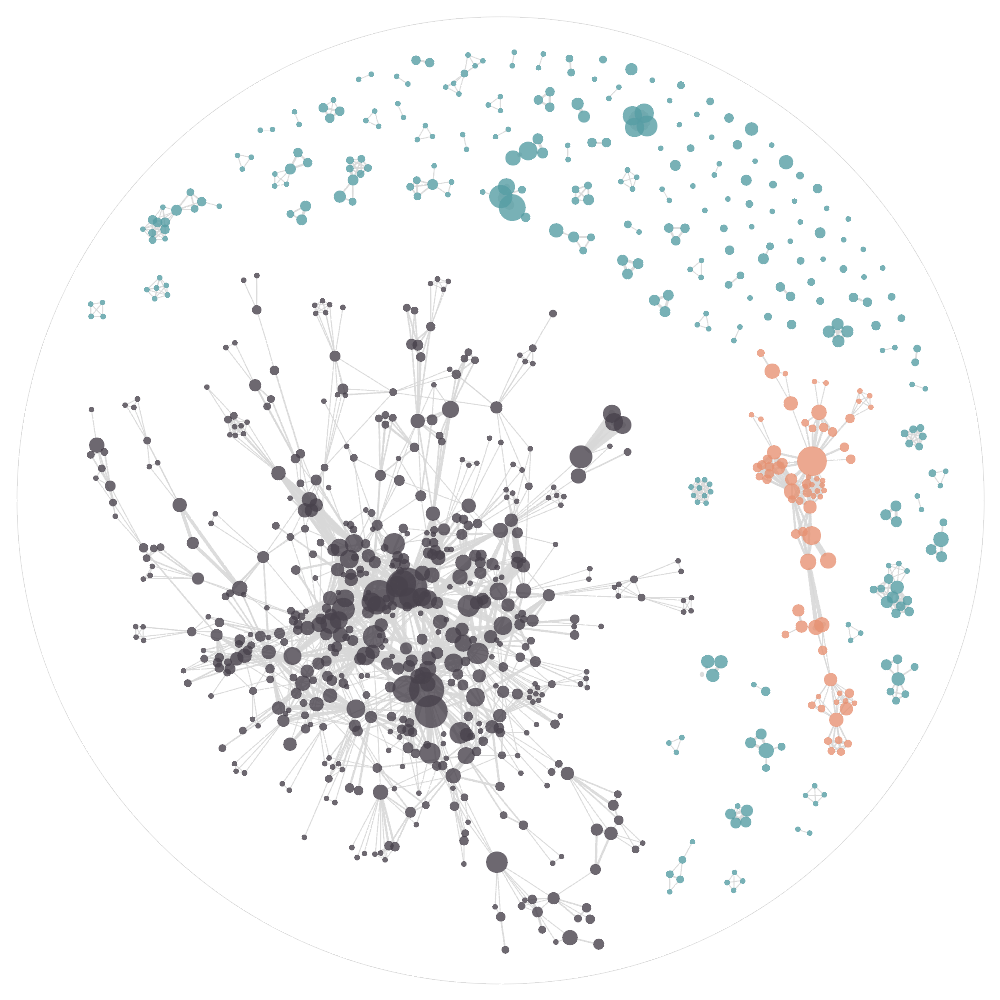
\includegraphics[width=6cm]{facebook_patents}

\end{columns}

\medskip

\centering 
\tiny{Source: Co-patenting network [\url{http://www.periscopic.com/news/exploring-innovation-signatures-in-patent-data}]}

\end{frame}

%------------------------------------------------

\begin{frame}
\frametitle{\insertsection}
\framesubtitle{Mapping collaborations (example)}

\centering
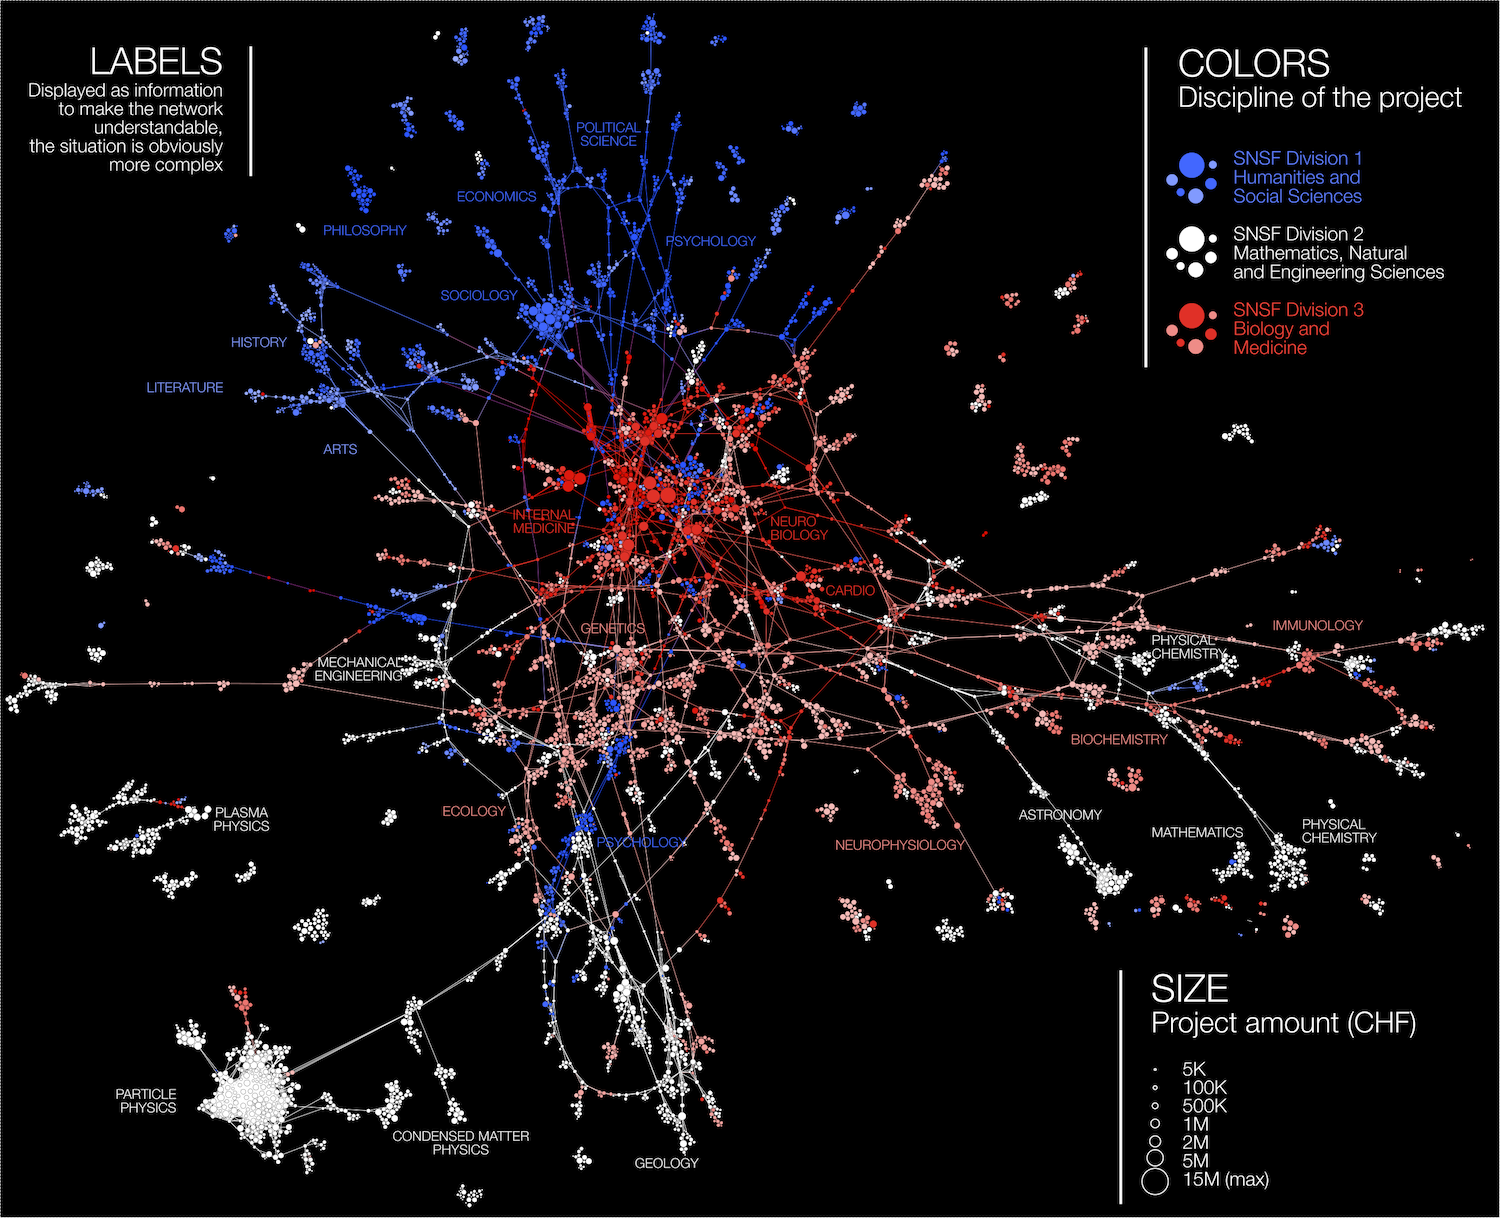
\includegraphics[width= 0.75\textwidth]{snf.png}\\
\tiny Source: SNSF-funded projects (2006-2015;, link representing shares of researchers) [\url{www.martingrandjean.ch/complex-network-visualisation-interdisciplinarity/}]

\end{frame}

%------------------------------------------------



%=======================================================	
% Mapping of cognitive connections
%=======================================================
\section{Mapping of cognitive connections}
%------------------------------------------------

\bgroup
\setbeamercolor{background canvas}{bg = navyblue}
\begin{frame}[plain]{}
\begin{center}
\color{white}{\Huge\insertsection}
\end{center}
\end{frame}
\egroup

%------------------------------------------------

\begin{frame}
\frametitle{\insertsection}
\framesubtitle{Cognitive connections}

Main scientometrics/bibliometrics {\color{blue}{mapping techniques}}
\begin{itemize}
\item Citation analysis
    \begin{itemize}
    \item Direct citation analysis \cite{Garfield1964}
    \item Co-citation analysis \cite{Small1973}
    \item Bibliographic coupling \cite{Kessler1963}
    \end{itemize}
\item Co-word analysis \cite{Callon1983}
\item Overlay mapping \cite{Rafols2010}
\end{itemize}

\end{frame}

%------------------------------------------------

\begin{frame}
\frametitle{\insertsection}
\framesubtitle{Citation analysis}

\centering
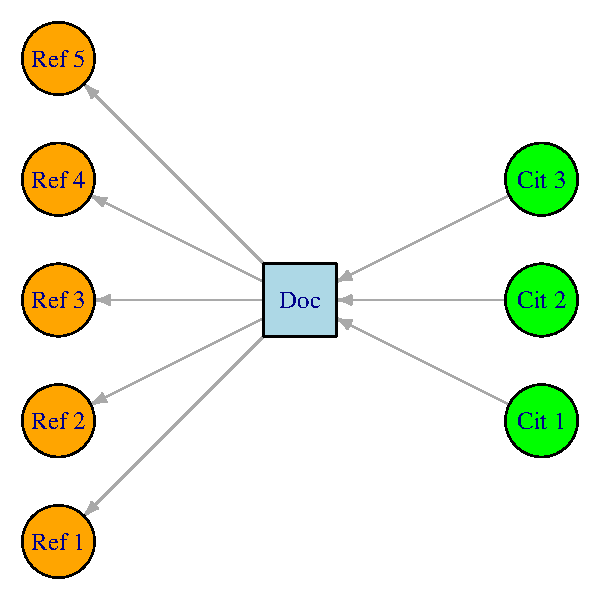
\includegraphics[width=0.80\textheight]{documents_citations}\\
\end{frame}

%------------------------------------------------

\begin{frame}
\frametitle{\insertsection}
\framesubtitle{Citation analysis}
\centering
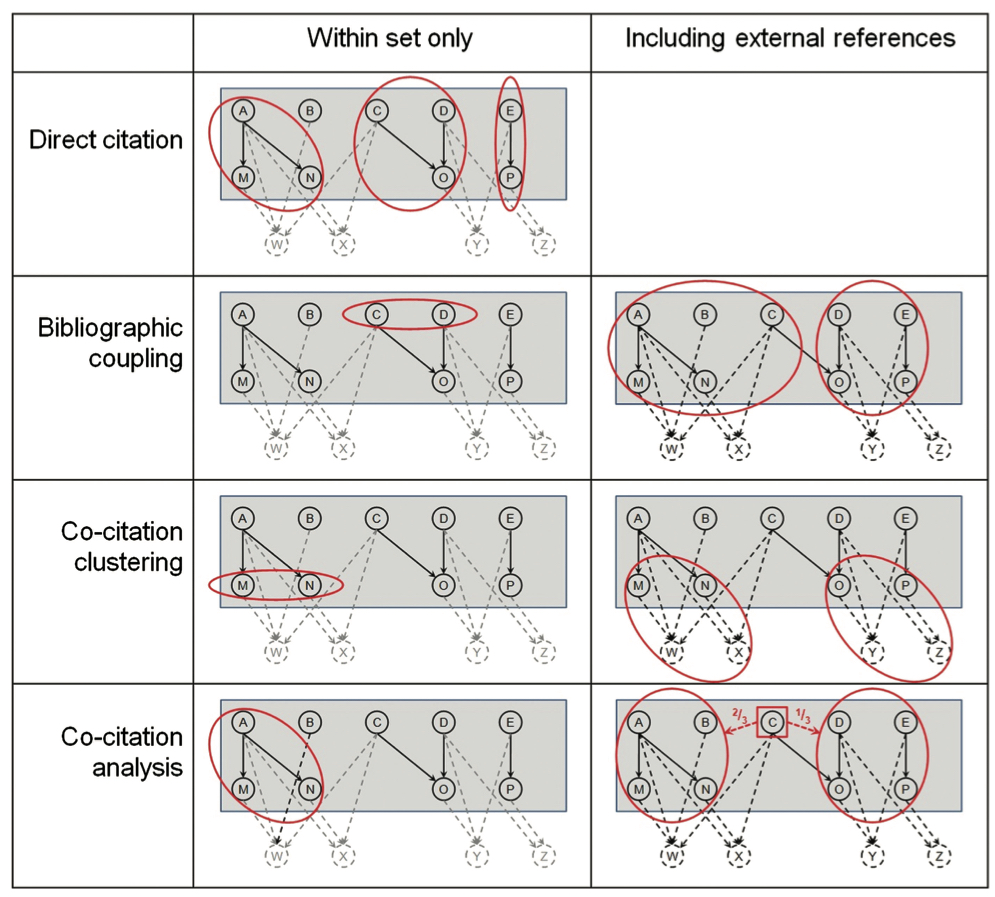
\includegraphics[height=0.8\textheight]{citation}\\
\tiny{Source: \cite{Boyack2010}}
\end{frame}

%NOTE=====
% Direct citation: requires long period of observations
% Articles A–E are recently published and not yet cited, 
% M–P are older and have been cited by the more recent documents in the set
% W–Z are not in thelongitudinal set, but have been cited by documents within the set
%
% Direct citation: cluster (A, M, N) will form because A cites both M and N; cluster (C, D, O) will form because C and D both cite O, and cluster (E,P) will form from the link between E and P. Article B will not be clustered because it does not cite any other article within the set
%
%Bibliographic coupling: only one cluster will form if only internal links are considered; cluster (C,D) forms since C and D both cite O
%
%Co-citation: co-citation clustering, which is simply the formation of clusters of co-cited documents, and co-citation analysis, which takes the result of co-citation clustering, and then assigns current papers (or papers from the research front) to the co-citation clusters
%
% Bibliographic coupling is able to cluster very recent papers but clusters fewer of the very old papers, while co-citation clustering does the opposite—it clusters the older papers, but cannot cluster the most recent papers that have not yet been cited. Direct citation clusters documents more evenly across the time window, and tends to cluster a larger number of documents than either bibliographic coupling or co-citation processes.
%
% Of the three pure citation-based approaches, bibliographic coupling slightly outperforms co-citation analysis using both accuracy measures; direct citation is the least accurate mapping approach by far.
%==========

%------------------------------------------------

\begin{frame}
\frametitle{\insertsection}
\framesubtitle{Direct citation analysis}

\centering
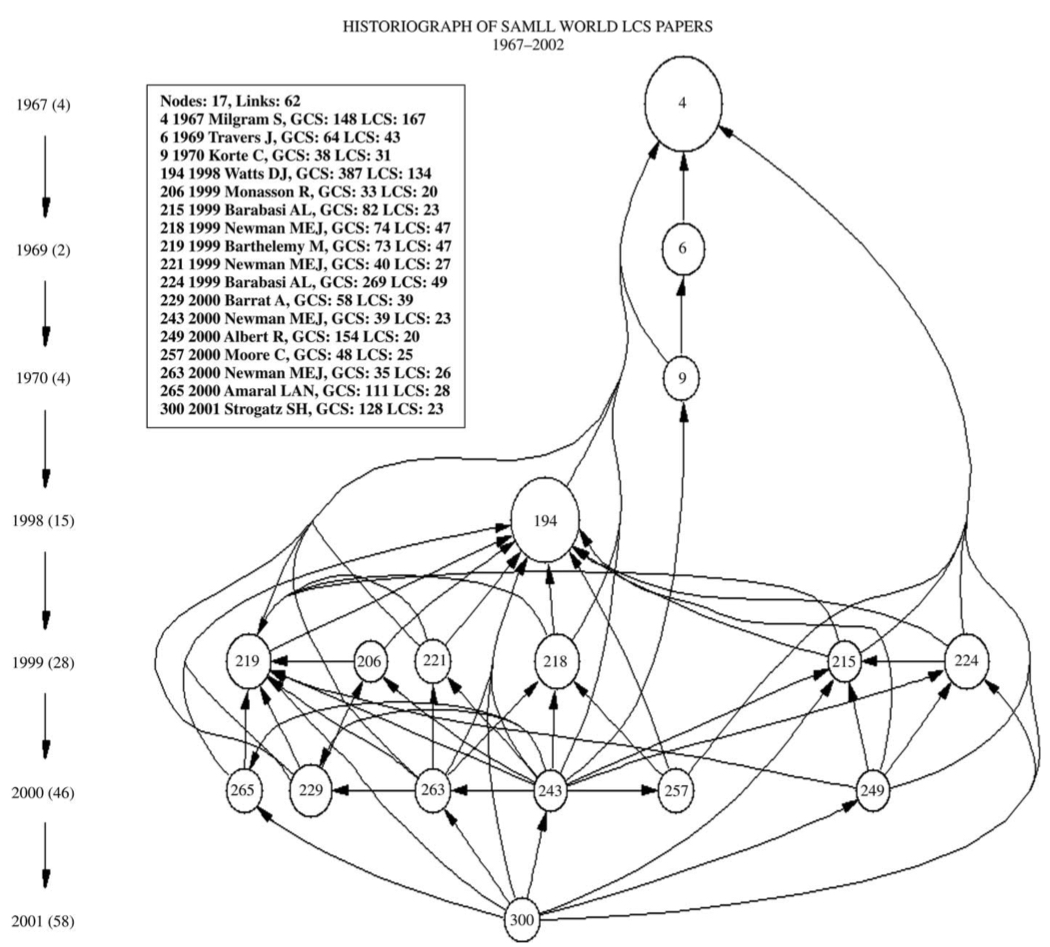
\includegraphics[height=0.8\textheight]{direct}\\
\tiny{Source: Literature on `Small World' \cite{Garfield2004}}

\end{frame}

%------------------------------------------------

\begin{frame}
\frametitle{\insertsection}
\framesubtitle{Co-citation analysis}

\centering
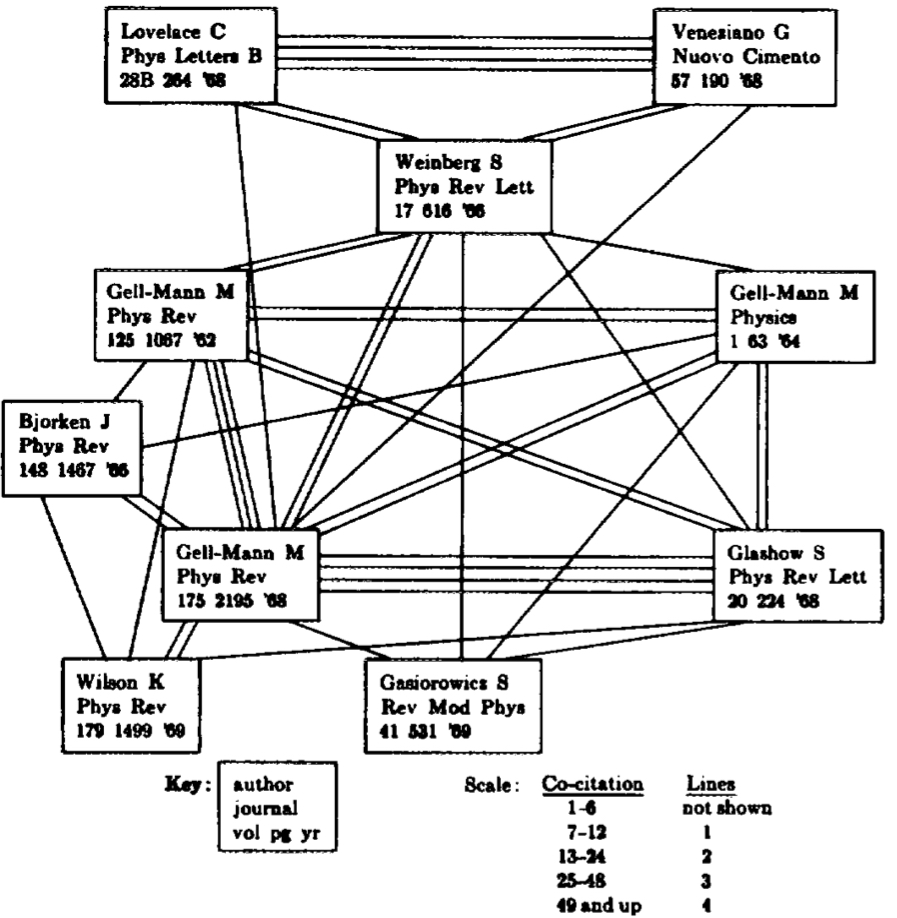
\includegraphics[height=0.8\textheight]{cocitation}\\
\tiny{Source: Co-citation of frequently cited papers in particle physics \cite{Small1973}}

\end{frame}

%------------------------------------------------

\begin{frame}
\frametitle{\insertsection}
\framesubtitle{Structural equivalence vs.\ regular equivalence}

\begin{itemize}
	\item {\color{blue}{Structural equivalence}}: nodes that share many network neighbours (e.g.\ documents cited by the same set of documents)
	\item  {\color{blue}{Regular equivalence}}: nodes that have neighbours that are similar to themselves (e.g.\ directors that have connections to their managers)
\end{itemize}


\centering
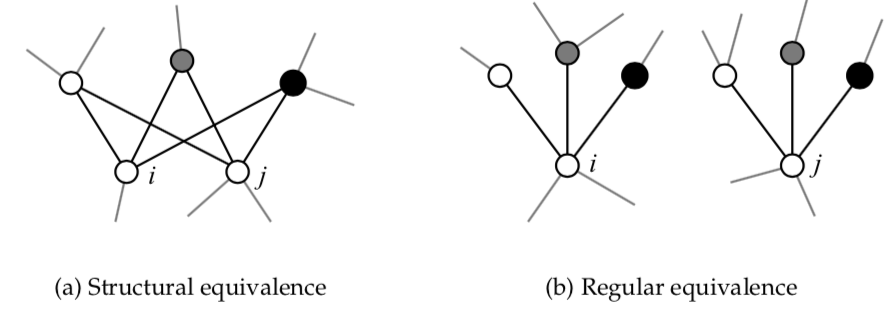
\includegraphics[width = 0.8\textwidth]{equivalence}\\
\tiny{Source: \cite{Newman2010}}

\end{frame}

%------------------------------------------------

\begin{frame}
\frametitle{\insertsection}
\framesubtitle{Cognitive distance}

To calculate the {\color{blue}{weight of cognitive connections}}, we focus on structural equivalence:

\bigskip

$\text{Co-occurrence} = n_{ij} = \sum_k A_{ik}A_{kj}$

\bigskip
  
$\text{Euclidean distance} = d_{ij} = \sqrt{\sum_k (A_{ik} - A_{jk})^2}$

\bigskip

$\text{Cosine similarity or Salton's cosine} = \sigma_{ij} = \frac{\sum_k A_{ik}A_{kj}}{\sqrt{\sum_k A_{ik}^{2}}\sqrt{\sum_k A_{kj}^{2}}}$


\end{frame}

%------------------------------------------------

\begin{frame}
\frametitle{\insertsection}
\framesubtitle{Cognitive distance}

\begin{center}
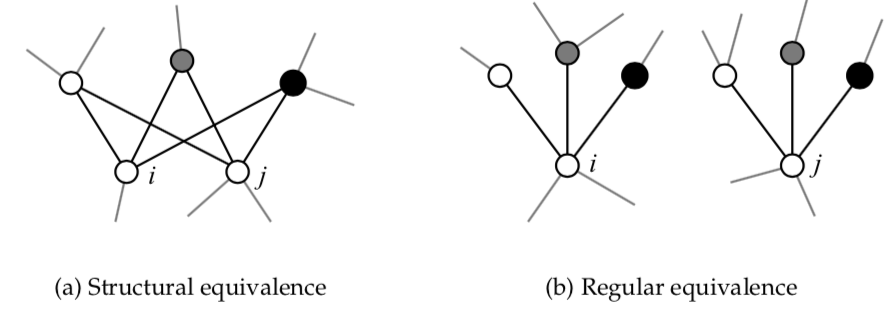
\includegraphics[width = 0.8\textwidth]{equivalence}\\
{\tiny Source: \cite{Newman2010}}
\end{center}

\medskip

Assuming the network to be undirected and unweighted:

\bigskip
 
$\text{Co-occurrence} = n_{ij} = \sum_k A_{ik}A_{kj} = 3$
	
\bigskip
  
$\text{Euclidean distance} = d_{ij} = \sqrt{\sum_k (A_{ik} - A_{jk})^2} = \sqrt{3} = 1.73$

\bigskip

$\text{Cosine similarity or Salton's cosine} = \sigma_{ij} = \frac{\sum_k A_{ik}A_{kj}}{\sqrt{\sum_k A_{ik}^{2}}\sqrt{\sum_k A_{kj}^{2}}} = \frac{3}{\sqrt{4}\sqrt{5}}=0.67 $

\end{frame}

%------------------------------------------------

\begin{frame}
\frametitle{\insertsection}
\framesubtitle{Co-citation analysis}

\centering
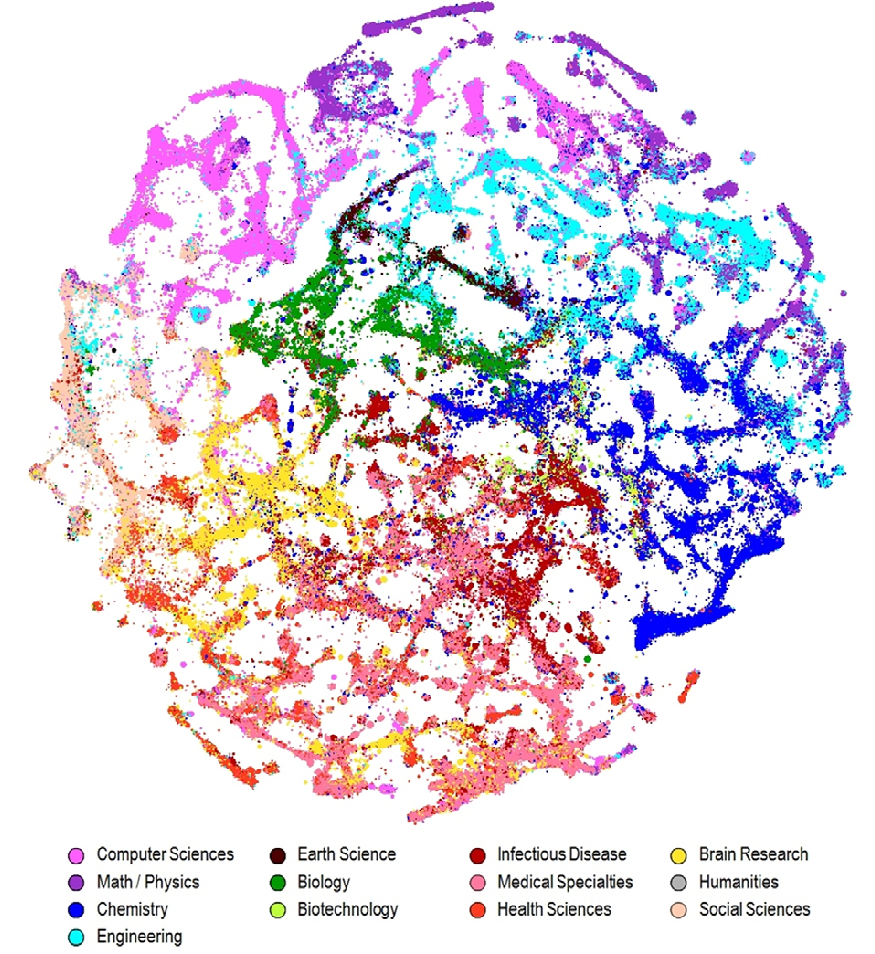
\includegraphics[height=0.8\textheight]{mapscience}\\
\tiny{Source: Map of Science (+20M articles and +2M patents from 1996-2011) \cite{Boyack2014}}

\end{frame}

%------------------------------------------------

\begin{frame}
\frametitle{\insertsection}
\framesubtitle{Co-word analysis}

\begin{columns}[c]


\column{.45\textwidth}
We can extract {\color{blue}{terms/keywords}}
\begin{itemize}
\item Title
\item Abstract
\item List of keywords
\item Full-text
\end{itemize}

\column{.45\textwidth}
\centering
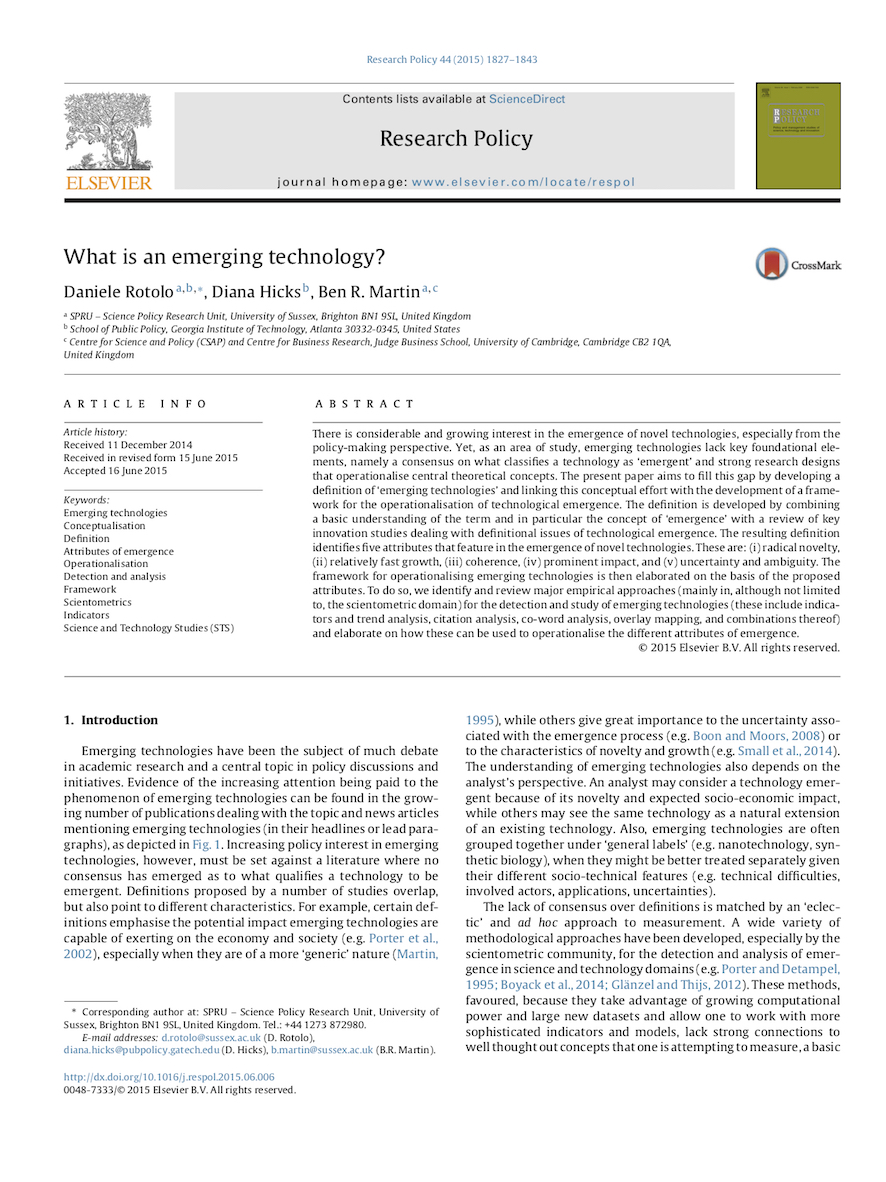
\includegraphics[width=4cm, frame]{paper}\\
\tiny{Source: \cite{Rotolo2015}}

\end{columns}

\end{frame}

%------------------------------------------------

\begin{frame}
\frametitle{\insertsection}
\framesubtitle{Co-word analysis}

\begin{columns}[c]

\column{.45\textwidth}

\centering
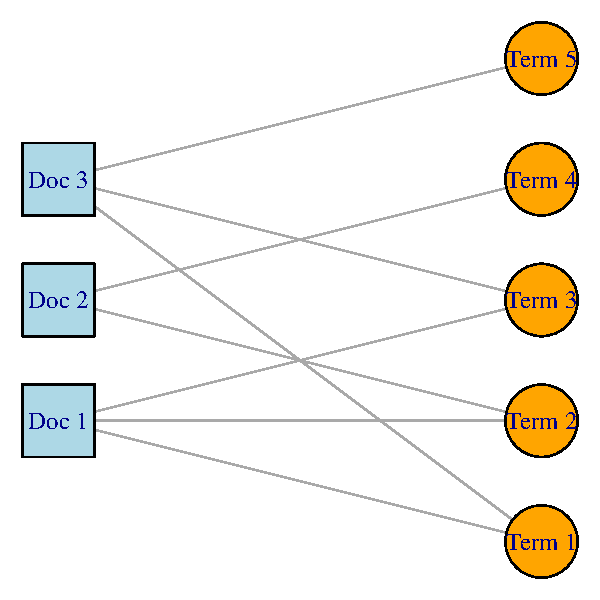
\includegraphics[width=0.80\textwidth]{documents_terms1}
\column{.45\textwidth}

\onslide<2>{
{\centering
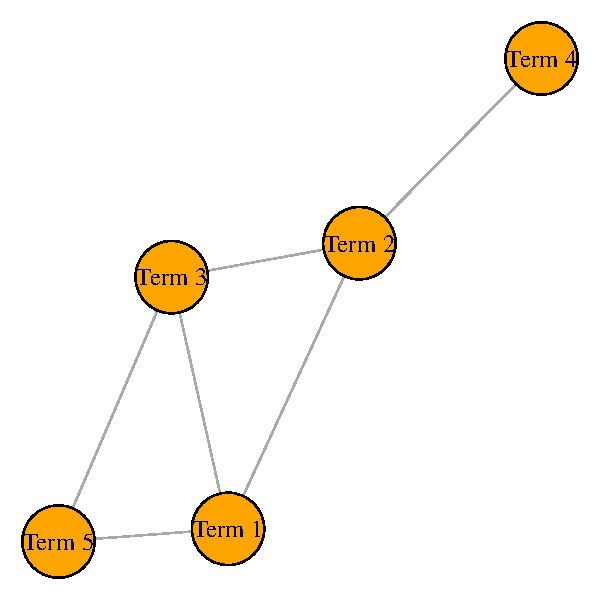
\includegraphics[width=0.80\textwidth]{documents_terms2}}

\medskip

{\color{blue}{Distances between terms}} using
\begin{itemize}
	\item co-occurrence
	\item euclidean distance
	\item cosine similarity
	\item ...
\end{itemize}}

\end{columns}

\end{frame}

%------------------------------------------------

\begin{frame}
\frametitle{\insertsection}
\framesubtitle{Co-word analysis}

\centering
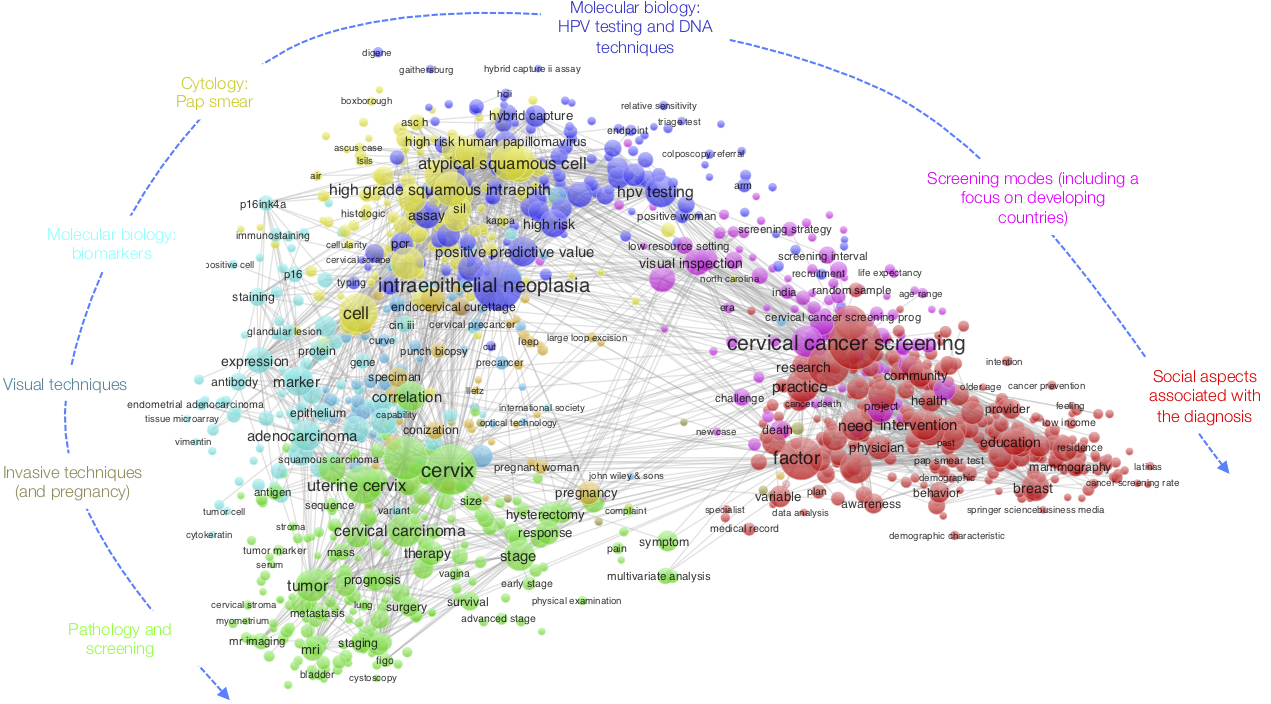
\includegraphics[height=0.75\textheight]{terms_map_cancer}\\
\tiny{Source: Terms extracted from the titles and abstracts of 4,921 publications on the diagnosis of cervical cancer (1980-2011 period)}

\end{frame}
%------------------------------------------------

\begin{frame}
\frametitle{\insertsection}
\framesubtitle{Co-word analysis}

\centering
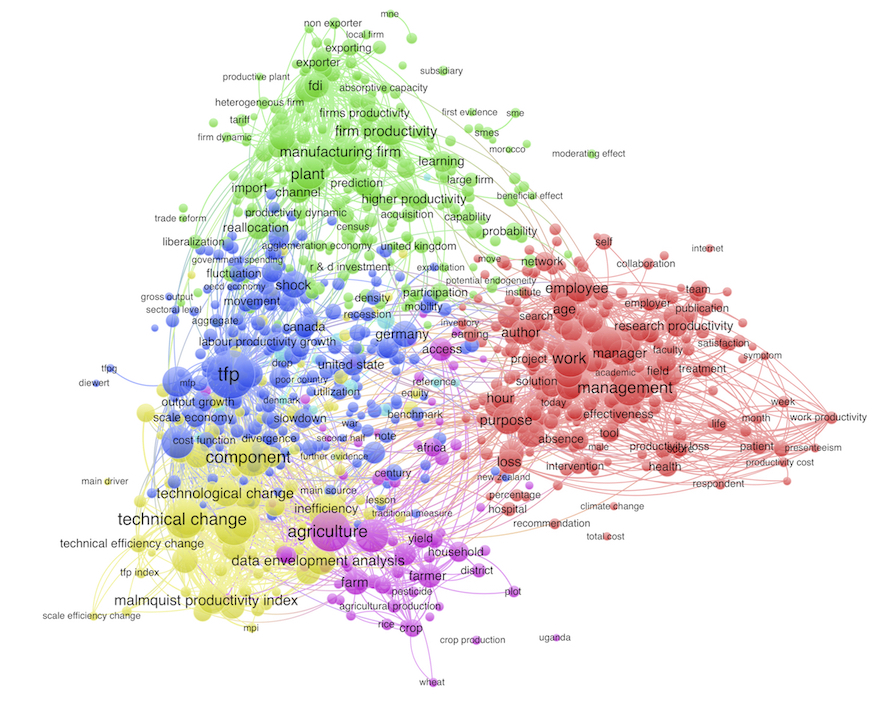
\includegraphics[height=0.75\textheight]{terms_map_productivity}\\
\tiny{Source: Terms extracted from the titles and abstracts of 6,676 articles in business, management, and economics research areas that included the term ``productivity'' in their titles (1957-2016 period)}

\end{frame}
%------------------------------------------------

\begin{frame}

\frametitle{\insertsection}
\framesubtitle{Overlay mapping}
\centering
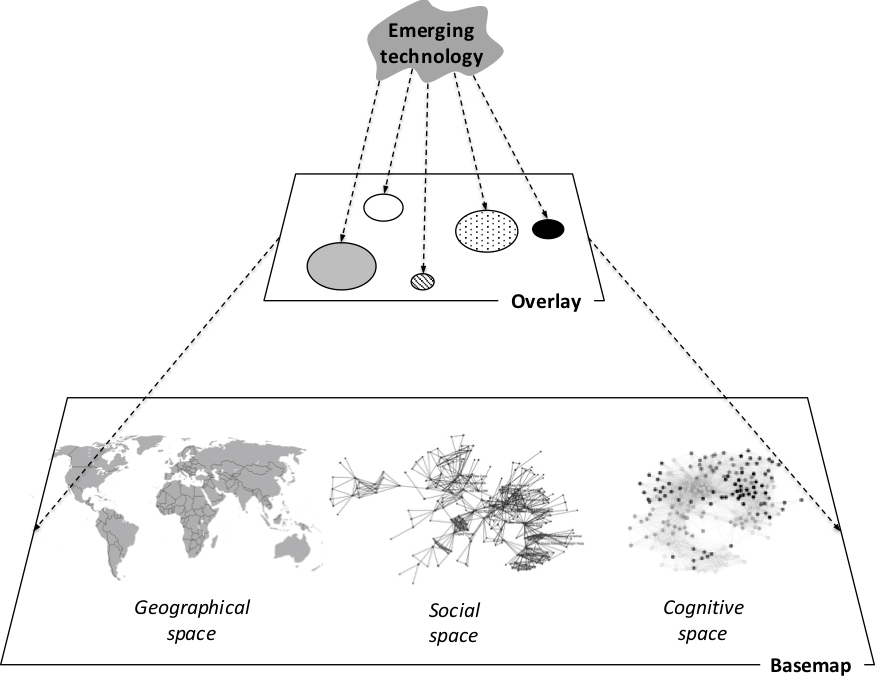
\includegraphics[width=\linewidth,height=0.75\textheight,keepaspectratio]{overlaymaps1}\\        
\tiny{Source: Overlay mapping \cite{Rotolo2017}}

\end{frame}
%------------------------------------------------

\begin{frame}

\frametitle{\insertsection}
\framesubtitle{Overlay mapping}
\centering
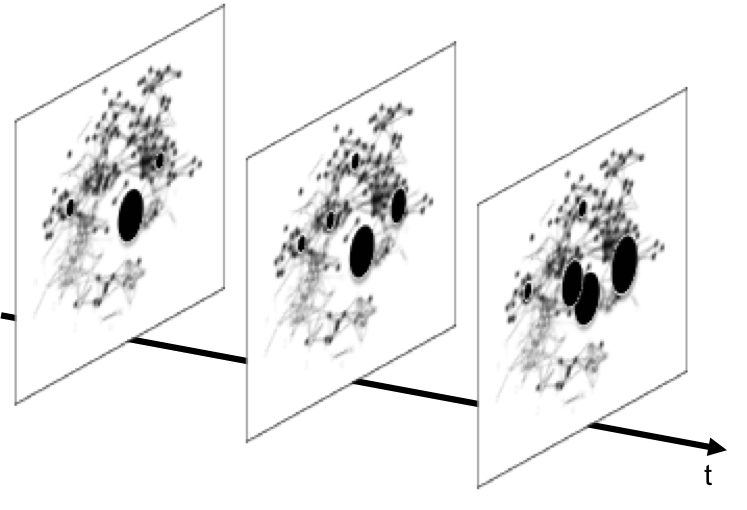
\includegraphics[width=\linewidth,height=0.50\textheight,keepaspectratio]{overlaymaps2}\\
\tiny{Source: Overlay mapping \cite{Rotolo2017}}

\end{frame}

%------------------------------------------------


\begin{frame}
\frametitle{\insertsection}
\framesubtitle{Overlay mapping}

A number of {\color{blue}{basemaps}} have been generated \cite{Rotolo2017}
\begin{itemize}
\item Geographical maps (e.g.\ Google Maps)
\item Disciplines (Subject Categories oft Web of Science)
\item Journals map
\item MeSH (Medical Subject Headings) map
\item IPC technological classes map (for patent data)
\end{itemize}

\end{frame}

%------------------------------------------------

\begin{frame}
\frametitle{\insertsection}
\framesubtitle{Overlay mapping}

\centering
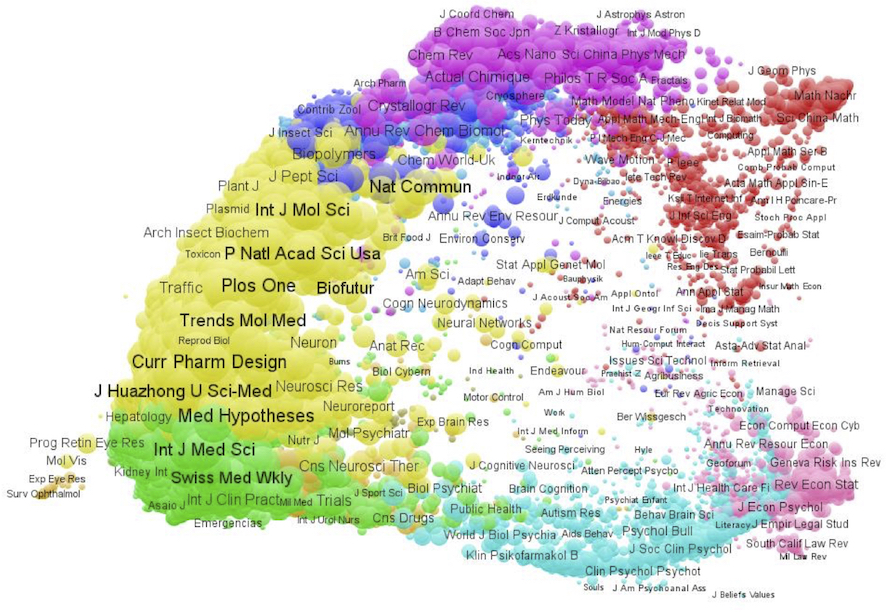
\includegraphics[width=\linewidth,height=0.75\textheight,keepaspectratio]{journals}\\
\tiny{Source: Journal basemap (+10,000 journals)  \cite{Leydesdorff2012b}}

\end{frame}

%------------------------------------------------

\begin{frame}
\frametitle{\insertsection}
\framesubtitle{Overlay mapping}


\begin{columns}

\column{.50\textwidth}
\centering
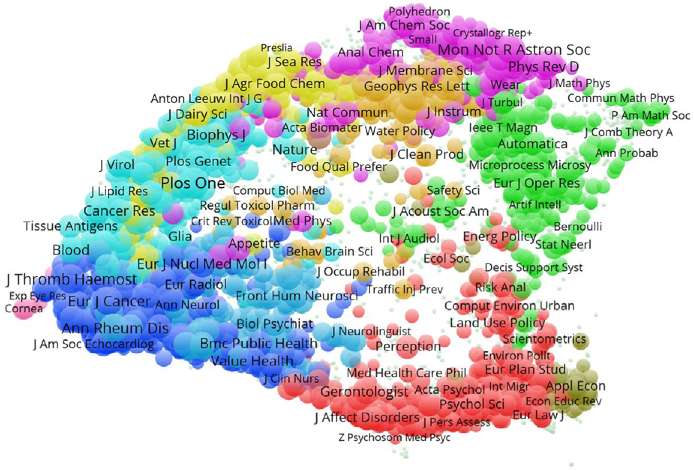
\includegraphics[width=\linewidth,height=0.50\textheight,keepaspectratio]{journals_NL}\\
\tiny{Netherlands (2013)}

\column{.50\textwidth}
\centering 
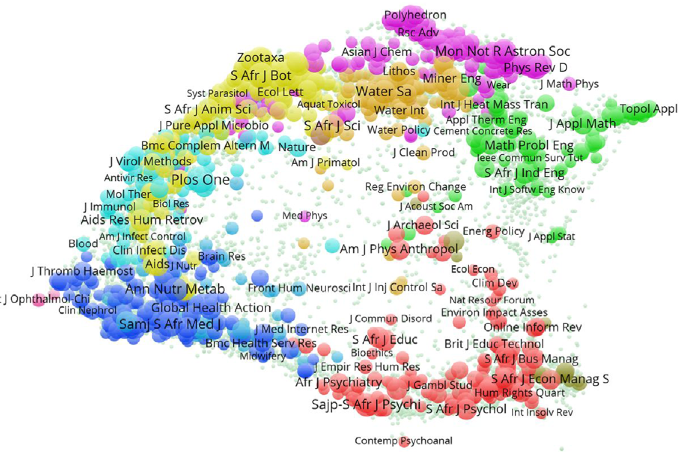
\includegraphics[width=\linewidth,height=0.50\textheight,keepaspectratio]{journals_SA}\\
\tiny{South Africa (2013)}

\end{columns}

\centering
\tiny{Source: Journal overlay map \cite{Leydesdorff2016}}
	
\end{frame}
%------------------------------------------------

\begin{frame}
\frametitle{\insertsection}
\framesubtitle{Overlay mapping}

\centering
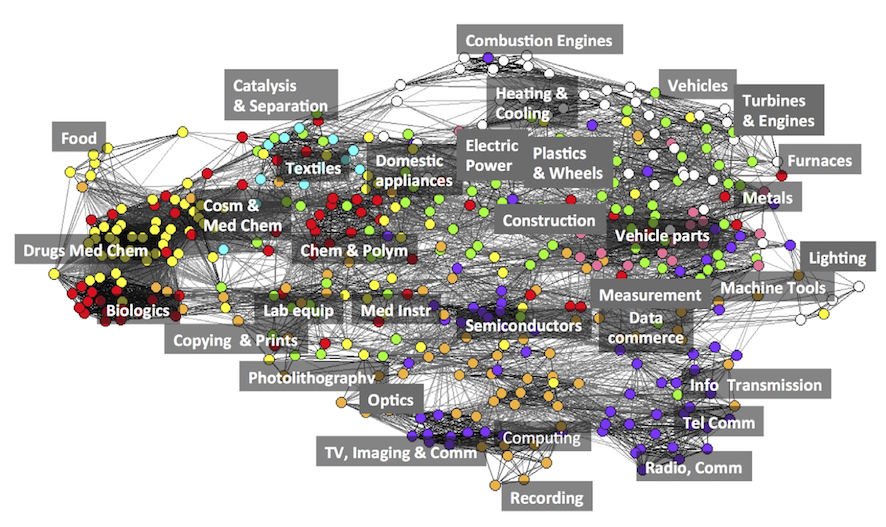
\includegraphics[width=\linewidth,height=0.75\textheight,keepaspectratio]{patent_map}\\
\tiny{Source: Patent basemap (466 IPC)  \cite{Kay2014}}

\end{frame}

%------------------------------------------------

\begin{frame}
\frametitle{\insertsection}
\framesubtitle{Overlay mapping}


\begin{columns}

\column{.50\textwidth}
\centering
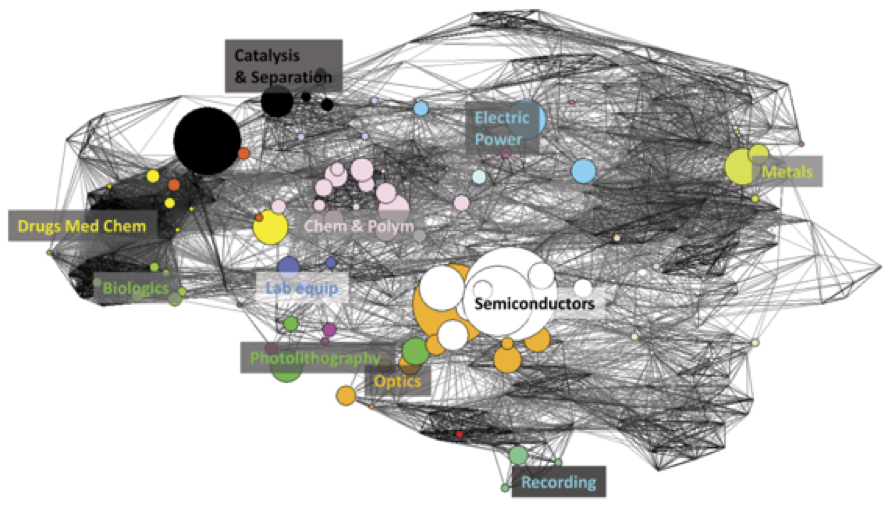
\includegraphics[width=\linewidth,height=0.50\textheight,keepaspectratio]{patent_Samsung}\\
\tiny{Samsung}

\column{.50\textwidth}
\centering 
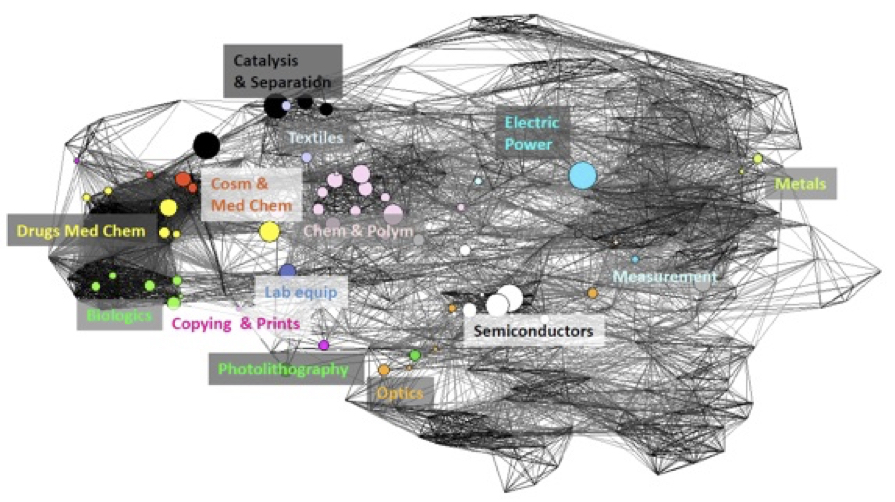
\includegraphics[width=\linewidth,height=0.50\textheight,keepaspectratio]{patent_Dupont}\\
\tiny{Dupont}

\end{columns}

\centering
\tiny{Source: Patent basemap and overlays \cite{Kay2014}}
	
\end{frame}
%------------------------------------------------









%=======================================================
%	Questions
%=======================================================
\bgroup
\setbeamercolor{background canvas}{bg = orange}
\begin{frame}[plain]{}
\begin{center}
\color{white}{\Huge Questions}
\end{center}
\end{frame}
\egroup




%%=======================================================
%	Next time ...
%%=======================================================
\section*{Next time ...}

%------------------------------------------------
\bgroup
\setbeamercolor{background canvas}{bg = navyblue}
\begin{frame}[plain]{}
\begin{center}
\color{white}{\Huge\insertsection}
\end{center}
\end{frame}
\egroup

%------------------------------------------------

\begin{frame}
\frametitle{\insertsection}

\begin{itemize}

\item \textbf{Seminar: Innovation networks}
	\begin{itemize}
	\item Practice with VOSViewer
	\end{itemize}
	
\medskip
\medskip

\item  \textbf{Lecture: Social network theories}
	\begin{itemize}
	\item Social capital
	\item Strength of weak ties
	\item Structural holes
	\end{itemize}	

		
\end{itemize}

\end{frame}

%------------------------------------------------











%=======================================================
%	References
%=======================================================
\begin{frame}[allowframebreaks]
\frametitle{References}
\tiny
\bibliographystyle{apalike}
\bibliography{/Users/dr213/Dropbox/References/bibtex_references/library.bib}
\end{frame}
%------------------------------------------------





\end{document}x§